
%If our lexical priors -- our global conventions -- serve as a source of stability in meaning over longer timescales, then what accounts for our extraordinary flexibility  over short timescales? How do we coordinate on efficient local conventions, or \emph{conceptual pacts}, for talking about things we've never talked about before? In this section, we review the dynamics of coordination within repeated reference games and explore the possibility, formalized in Chapter 2, that rapid adaptation can be understood in a Bayesian modeling framework as lexical inference given partner-specific data.%: $P(\mathcal{L}_i | D_i, \Theta)$. 

We begin with the phenomenon of increasing efficiency in repeated reference games: speakers use detailed descriptions at the outset but converge to increasingly compressed shorthand while remaining understandable to their partner.
While this phenomenon has been extensively documented, to the point of serving as a proxy for measuring common ground, it has continued to pose a challenge for computational models of language use.
One simple explanation --- that it is merely an effect of familiarity or repetition on the part of the speaker, not related to \emph{ad hoc} conventions --- can be easily dismissed. 
When participants are asked to repeatedly refer to the same targets for a \emph{hypothetical} partner, no decrease in utterance length is found; in some cases utterances actually get longer \cite{HupetChantraine92_CollaborationOrRepitition}. 
This control experiment suggests that whatever is changing must be a result of the \emph{interaction} between partners.

It is also not clear how increasing efficiency could be explained by the lower-level alignment mechanisms proposed in \emph{interactive alignment} accounts \cite{pickering2004toward, pickering2006alignment, garrod2009joint}.
According to these accounts, coordination on meaning proceeds primarily through automatic priming at lower levels of representation.
While low-level priming is certainly possible in repeated reference tasks, especially when listeners engage in extensive dialogue or alternate in the speaker role, it is not clear why priming would favor some words in a long referring expression over others, or lead to increasing efficiency.
Furthermore, priming alone cannot explain why speakers still converge to more efficient labels even when the listener is prevented from saying anything at all and only indirect feedback about the listener's response accuracy is provided \cite{KraussWeinheimer66_Tangrams}; conversely, speakers continue using longer descriptions given non-verbal evidence of errors \cite{hawkins2020characterizing}.
In these cases, there are no linguistic features available for priming or alignment.
Explaining when and why speakers believe that shorter descriptions will suffice requires a mechanism for coordination on meaning even given sparser, non-verbal feedback.

Finally, we consider agent-based models implementing simple update rules \cite{steels_self-organizing_1995,barr_establishing_2004,young_evolution_2015}.
These models all share some mechanism that makes utterances more likely to be produced after communicative successes and less likely after communicative failures, as in Roth-Erev reinforcement learning \cite{erev1998predicting}.
While this form of reinforcement is a powerful mechanism for allowing groups to reach consensus, it is not clear why an agent using such rules would initially prefer to produce longer utterances, or how reinforcing initially long descriptions could lead to reduction. % without some mechanism for \emph{credit assignment} to the component words.
When reduction has been investigated in these models (e.g. as in the phenomenon of phonological erosion), the process has simply been hard-coded as an $\epsilon$ probability of speakers dropping a token \cite{beuls2013agent,steels2016agent}.

In this section, we argue that our Bayesian account provides a natural computational explanation for increasing efficiency in terms of the inferences made by speakers.
Given that this phenomenon arises in purely dyadic settings, it also provides an opportunity to explore more basic properties of the first two capacities formalized in our model (\emph{uncertainty} and \emph{partner-specific learning}) before introducing the fully hierarchical component in later sections. 
In brief, we show that increasing efficiency emerges from the Gricean maxim of quantity, as formalized in the speaker's tradeoff between informativity and parsimony (Eq.~\ref{eq:marginalized}), under shifts in their uncertainty about the listener's language model. 
For novel, ambiguous objects like tangrams, where speakers do not expect strong referential conventions to be shared, longer initial descriptions are motivated by high initial uncertainty in the speaker's lexical prior $P(\phi_k | \Theta)$. 
Combining multiple partially redundant descriptors hedges against the possibility that particular meanings are not shared by the listener.
As the interaction goes on, the speaker obtains feedback $D_k$ from the listener responses and updates their posterior beliefs $P(\phi_k | D_k)$ accordingly. 
As uncertainty gradually decreases, they are able to achieve the same expected informativity with shorter, more efficient messages. 

\subsection{Model simulations}

\begin{figure}
\centering
    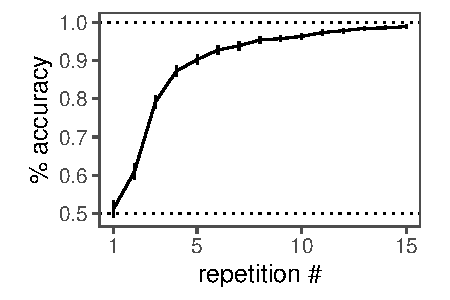
\includegraphics[scale=1]{sec1-convergence.pdf}
  \caption{\emph{Agents learn to successfully coordinate over repeated interactions.} Error bars are bootstrapped 95\% CIs.}
  \label{fig:sec1model}
\end{figure}

  \begin{figure*}
\centering
    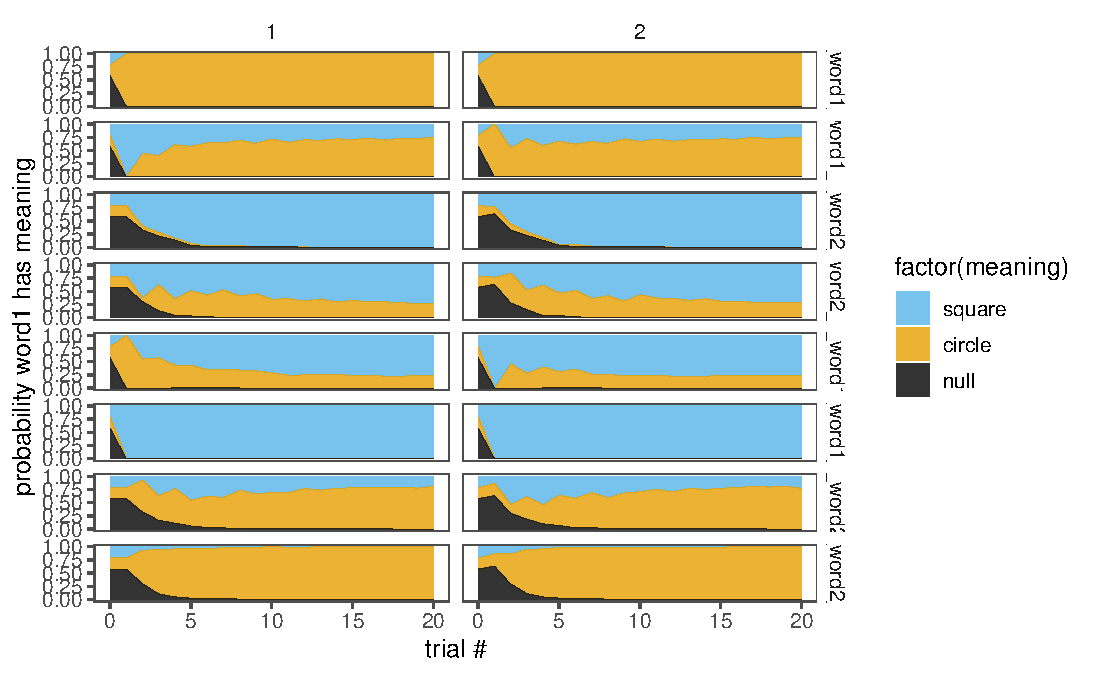
\includegraphics[scale=.9]{sec1-arbitrariness}
    \vspace{1em}
  \caption{\emph{Path-dependence of conventions.} The trajectory of each agent's beliefs about $\phi(u_1)$ in Simulation 1.1 are shown following all possible outcomes of the first trial. The top four rows are cases where the listener happened to correctly choose the target. In these cases, agents condition on the same data and rapidly converge on a system of meaning consistent with this feedback, e.g. when $u_1$ was successfully used to refer to the circle (shown in orange), both agents subsequently believe that $u_1$ means \emph{circle}. The bottom four rows show cases where the listener initially chooses the incorrect object. In these cases, the agents condition on different data (reflected in diverging beliefs on trial 2) but ultimately recover from this mis-coordination depending on subsequent rounds.}
  \label{fig:path-dependence}
\end{figure*}

\paragraph{Simulation 1.1: Coordination}

We build up to our explanation of increasing efficiency through a series of simpler simulations.
The first of these simulations demonstrates the most fundamental desideratum for any model of \emph{ad hoc} coordination: agents equipped with our inferential machinery are able to coordinate on a communication system in the absence of shared priors. 
We consider the simplest possible reference game with two objects, $\mathcal{O} = \{o_1, o_2\}$, where the speaker must choose between two one-word utterances $\mathcal{U} = \{u_1, u_2\}$ with equal production cost. 

To define the agents' initial lexical prior $P(\phi)$ over the expected meanings of each utterance, we must first say what representation we are using for the agents' lexicon $\mathcal{L}_{\phi}$.
For simplicity, we follow prior Bayesian models of word learning \cite<e.g.>{XuTenenbaum07_WordLearningBayesian} and represent the space of meanings for an utterance as the set of nodes in a concept taxonomy\footnote{There are many alternative representational choices compatible with our core model, including parameterized vector embeddings and multi-layer neural networks, which may be more appropriate for scaling our model to larger spaces of words and referents. We return to these possibilities in the General Discussion.}.
When objects are conceptually distinct, as assumed in most prior models of signaling games, this taxonomy is flat and the target space of utterance meanings is simply equivalent to the space of individual objects, i.e.~$\den{u}_{\phi} = \phi(u) \in \mathcal{O}$ for all $u\in\mathcal{U}$. 
Then the lexical meaning function is defined to be
$$
\mathcal{L}_\phi(o,u) = \left\{ \begin{array} {rl} 1 & \textrm{if $\phi(u)=o$} \\ 0 & \textrm{otherwise} \end{array}\right.
$$
To explore pure coordination, we initialize agents with uniform priors: $$\phi(u_i) \sim \textrm{unif}\{o_1, o_2\}$$ for all $u_i \in \mathcal{U}$.

The first step of interaction proceeds as follows.
Suppose the target object on the first round is $o_1$.
Due to the uniform priors, both utterances are equally likely to apply to either object. 
Because each utterance is equally (un)informative, the speaker must randomly sample an utterance $u~\sim~S(u|o_1)$ --- say, $u_1$.
They may then observe the listener's selection of an object $o \sim L(o | u_1)$ --- say, $o_1$, a correct response.
Finally, they may use the observed pair $D = \{u_1, o_1\}$ to update their beliefs about the listener's true lexicon $P(\phi | D)\propto L_1(o_1 | u_1, \phi)P(\phi)$.
The listener is similarly able to update their beliefs about the speaker's true lexicon $P(\phi | D)\propto S_1(u_1 | o_1, \phi)P(\phi)$. 
Both agents then proceed to the next trial, where they use this posterior distribution to produce or interpret language.

To examine how the dynamics of this process unfold over multiple rounds, we conducted a simulation running these models forward for 1000 different trajectories.
We have the agents swap speaker and listener roles on each trial, and randomly sample the target on each trial from the set of $\{o_1, o_2\}$.
We use enumeration to exactly compute each agent's posterior beliefs about $\phi$ at each time step.
Trajectories diverge when different actions are sampled at a time step.
For example, if the speaker had sampled $u_2$ instead of $u_1$ on the first trial, or if the listener had made an error by choosing $o_2$, then they would subsequently condition on these observations instead.

We highlight several key results from these simulations at soft-max optimality parameter values $w_L = w_S = 16$ and memory discounting parameter $\beta = 0.8$ (see Appendix Fig.~\ref{fig:arbitrariness_grid} for an exploration of other values).
First, most fundamentally, the communicative success of the dyad rises over the course of interaction; the listener is able to more accurately select the true target object (see Fig.~\ref{fig:sec1model}). 
Second, the initial symmetry between the meanings is broken by initial choices, leading to \emph{arbitrary} but \emph{stable} mappings in future rounds.
This can be seen by examining the path-dependence of beliefs following all possible outcomes of the initial trial (see Fig.~\ref{fig:path-dependence}). 
Third, because each agent assumes their partner is using language cooperatively, they can also make inferences about \emph{unheard} utterances. 
Observing $D = \{(u_2, o_1)\}$ also provides evidence that $u_1$ is \emph{not} a good fit for $o_1$ (e.g. see third row of Fig.~\ref{fig:path-dependence}).
This effect arises from Gricean pragmatic reasoning: if $u_2$ were a better fit for $o_1$, the speaker would have used it instead \cite{Grice75_LogicConversation}. 
Fourth, conventions may form based on \emph{failed references} as well as successful ones: if the speaker intends $o_1$ and says $u_1$, but then the listener incorrectly picks $o_2$, the speaker will take this as evidence that $u_1$ actually means $o_2$ in their partner's lexicon and become increasingly likely to use it that way on subsequent rounds.

\paragraph{Simulation 1.2: Efficiency}

\begin{figure*}
\centering
    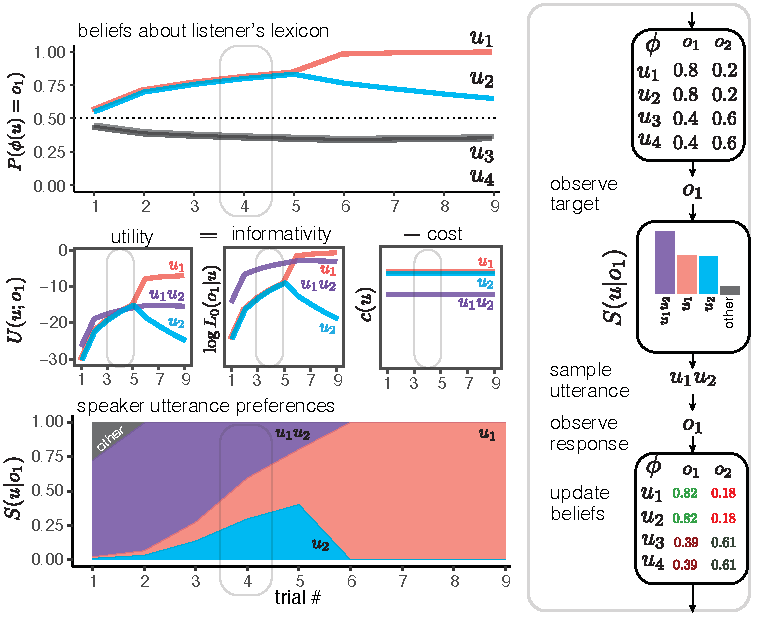
\includegraphics[scale=1.2]{sec1-reduction_example}
  \caption{\emph{Agent converge on more efficient utterances over repeated interactions.}}
  \label{fig:sec1efficiency}
\end{figure*}


Next, we show how our model explains reduction of utterance length over multiple interactions. 
For utterances to be reduced, of course, they must vary in length, so we extend our grammar to include \emph{conjunctions}. 
Conjunctions are one of the simplest ways to construct longer, non-atomic utterances compositionally from lexical primitives, using the product rule \cite<see also>[who instead consider negation]{SteinertThrelkeld16_CompositionalSignaling}:
$$\mathcal{L}_\phi(u_iu_j, o) = \mathcal{L}_\phi(u_i, o) \times \mathcal{L}_\phi(u_j, o)$$
We consider a scenario where two objects $\{o_1, o_2\}$ differ along two different features. 
The speaker thus has four primitive words at their disposal -- two words for the first feature ($\{u_{11}, u_{12}\}$) and two for the second $\{u_{21}, u_{22}\}$. 
While we established in the previous section that conventions can emerge over a reference game in the complete absence of initial preferences, players often bring such preferences to the table. 
A player who hears `ice skater' on the first round of a tangrams task is more likely to select some objects more than others, even though they still have some uncertainty over its meaning in the context. 
To show that our model can accommodate this fact, we allow the speaker's initial prior meanings to be slightly biased. 
We assume $u_{11}$ and $u_{21}$ are a priori more likely to mean $o_1$ and $u_{12}$ and $u_{22}$ are more likely to mean $o_2$.

\begin{figure}
\centering
    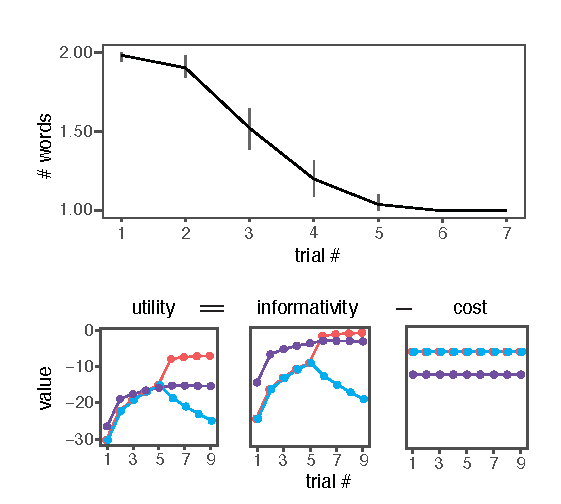
\includegraphics[scale=1]{sec1-efficiency-explanation}
  \caption{\emph{Agent converge on more efficient utterances over repeated interactions.} (A) Results of simulation 1.2. Error bars are bootstrapped 95\% CIs. (B) More efficient utterances gradually gain in utility as a tradeoff between informativity and efficiency.}
  \label{fig:sec1efficiency}
\end{figure}


We ran 1000 forward samples of 6 rounds of speaker-listener interaction, and averaged over the utterance length at each round \footnote{In our simulations, we used $\alpha = 10$ but found the basic reduction effect over a range of different biases}. 
Our results are shown in Figure \ref{fig:sec1efficiency}: the expected utterance length decreases systematically over each round. 
To illustrate in more detail how this dynamic is driven by an initial rational preference for redundancy relaxing as reference becomes more reliable, we walk step-by-step through a single trajectory. 
Consider a speaker who wants to refer to object $o_1$. 
They believe their knowledgeable partner is slightly more likely to interpret their language using a lexicon in which $u_{11}$ and $u_{12}$ apply to this object, due to their initial bias. 
However, there is still a reasonable chance that one or the other alone actually refers more strongly to $o_2$ in the true lexicon. 
Thus, it is useful to produce the conjunction "$u_{11}$ and $u_{12}$" to hedge against this possibility, despite its higher cost. 
Upon observing the listener's response (say, $o_1$), the evidence is indeterminate about the separate meanings of $u_{11}$ and $u_{12}$ but both become increasingly likely to refer to $o_1$. 
In the trade-off between informativity and cost, the shorter utterances remain probable options. 
Once the speaker chooses one of them, the symmetry collapses and that utterance remains most probable in future rounds. 
In this way, meaningful sub-phrases are omitted over time as the speaker becomes more confident about the true lexicon. 

%\paragraph{Model comparison}
%
%Here we compare this model to several simpler baselines to establish which components of the model are necessary and sufficient for the desired behavior.
%
%\rdh{e.g., no pragmatics, pragmatics only in learning rule or only in decision rule instead of both, simpler pragmatics (reasoning about $L_0$ instead of $L_1$), point estimate instead of uncertainty, effect of different parameter regimes.} 
%
%\rdh{It may also be useful to explicitly show that the simpler Roth-Erev RL updating from this literature doesn't reduce, or even better show that this kind of simpler update rule is equivalent to something within our framework as a point estimate representation with maximum likelihood or something...?}

%In the limit, it doesn't matter whether you have pragmatics in both learning rule or decision rule. 
%In case where it's only in production rule, you'll produce the data with the necessary biases in learning.



\subsection{Discussion}

The explanation for increasing efficiency we have offered is consistent with some additional observations from prior empirical work.
For example, if participants reduce their lexical uncertainty over successive rounds, as we suggest, then we might expect a corresponding decrease in explicit markers of this uncertainty. 
Indeed, \citeA{BrennanClark96_ConceptualPactsConversation} counted \emph{hedges} across repetitions.
Hedges are expressions like \emph{sort of} or \emph{like}, and morphemes like \emph{-ish}, that explicitly mark uncertainty or provisionality, such as \emph{a car, sort of silvery purple colored} \cite{BrennanClark96_ConceptualPactsConversation,Fraser10_Hedging,MedlockBriscoe07_HedgeClassification}.
\citeA{BrennanClark96_ConceptualPactsConversation} found a much greater occurrence of hedges on the first round than the final round (26\% and 2\%, respectively).
Additionally, very few hedges were found on early trials in less ambiguous contexts (e.g. referring to a shoe in the context of dogs and fish), lending support for the specific use of hedges to mark uncertainty rather than a generic social use when first beginning to talk with a new partner.

\todo[inline]{Discuss specific relationships to other models, e.g. also the observation about }
While simple reinforcement learning models It is plausible that reinforcement learning models using more sophisticated algorithms could predict patterns of reduction with the addition of a cost term. 
For instance, neural network architectures appropriately incorporating compositionality and recurrence into production may be able to implicitly ground shorter utterances in prior usage using gradient-based learning \cite{hawkins2019continual}.
However, such a scheme would be much closer in spirit to our model.
We return to this issue in our discussion of the scalability of our model in the General Discussion.

Finally, our simulations in this section are consistent with recent analyses of exactly \emph{what} gets reduced \cite{hawkins2020characterizing}.
Is the speaker adopting a fragment shorthand by randomly and noisily dropping words, or are they simplifying or narrowing their descriptions to names by systematically omitting redundant details?
Closed-class parts of speech like determiners and prepositions \emph{are} much more likely to be dropped than open-class parts of speech like adjectives and nouns, and entire modifying clauses are more likely to be dropped together than expected by random corruption.
This accords with early hand-tagged analyses by \citeA{Carroll80_NamingHedges}, which found that in three-quarters of transcripts from \citeA{krauss_changes_1964} the short names that participants converged upon were prominent in some syntactic construction at the beginning, often as a head noun that was initially modified or qualified by other information. 
These more fine-grained analyses suggest that reduction is grounded in the prior lexical content of the interaction and the speaker's increasing confidence in how the listener will interpret an initially ambiguous label. 

